\begin{figure}[H]
	\centering
	\usetikzlibrary{positioning,arrows.meta}
	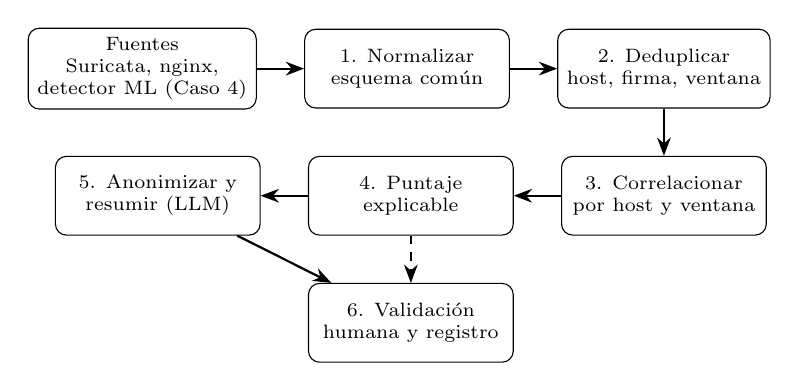
\begin{tikzpicture}[node distance=6mm,
		box/.style={draw, rounded corners, align=center, font=\scriptsize, minimum width=26mm, minimum height=10mm},
		arr/.style={-{Stealth}, thick}]
		\node[box] (src) {Fuentes\\Suricata, nginx,\\detector ML (Caso 4)};
		\node[box, right=of src] (norm) {1. Normalizar\\esquema común};
		\node[box, right=of norm] (dedup) {2. Deduplicar\\host, firma, ventana};
		\node[box, below=of dedup] (corr) {3. Correlacionar\\por host y ventana};
		\node[box, left=of corr] (score) {4. Puntaje\\explicable};
		\node[box, left=of score] (llm) {5. Anonimizar y\\resumir (LLM)};
		\node[box, below=of score] (human) {6. Validación\\humana y registro};
		\draw[arr] (src)--(norm); \draw[arr] (norm)--(dedup); \draw[arr] (dedup)--(corr);
		\draw[arr] (corr)--(score); \draw[arr] (score)--(llm); \draw[arr] (llm)--(human);
		\draw[arr, dashed] (score)--(human);
	\end{tikzpicture}
	\caption{Pipeline de correlación y priorización de alertas del Caso 9.}
	\label{fig:c9_pipeline}
\end{figure}
